%!TEX program = xelatex
\documentclass[nohyper,nobib]{tufte-handout}
\XeTeXinputnormalization=1
\usepackage{fontspec}
\usepackage[babel,german=quotes]{csquotes}
\usepackage{polyglossia}
\setdefaultlanguage[spelling=new,babelshorthands=true]{german}
\setotherlanguage[]{english}
\usepackage[xetex,bookmarks=true,colorlinks=true,linktoc=section,]{hyperref}
% \usepackage{hyphenat}

\usepackage{booktabs}
\usepackage{amsmath}
\usepackage{color}

% tufte fix
\ifxetex
  \newcommand{\textls}[2][5]{%
    \begingroup\addfontfeatures{LetterSpace=#1}#2\endgroup
  }
  \renewcommand{\allcapsspacing}[1]{\textls[15]{#1}}
  \renewcommand{\smallcapsspacing}[1]{\textls[10]{#1}}
  \renewcommand{\allcaps}[1]{\textls[15]{\MakeTextUppercase{#1}}}
  \renewcommand{\smallcaps}[1]{\smallcapsspacing{\scshape\MakeTextLowercase{#1}}}
  \renewcommand{\textsc}[1]{\smallcapsspacing{\textsmallcaps{#1}}}
\fi

\newcommand{\adjustimg}{% Horizontal adjustment of image
  \checkoddpage%
  \ifoddpage\hspace*{\dimexpr\evensidemargin-\oddsidemargin}\else\hspace*{-\dimexpr\evensidemargin-\oddsidemargin}\fi%
}
\newcommand{\centerimg}[2][width=\textwidth]{% Center an image
  \makebox[\textwidth]{\adjustimg\includegraphics[#1]{#2}}%
}

\author{Jakob Schmolling}
\date{\today}

% \usepackage{hyphenat} 
\usepackage[
	% sorting=nyt,
	style=alphabetic,
	% citestyle=alphabetic,
	natbib=false,
	%style=verbose,
  autocite=footnote,
  backend=biber
	]{biblatex}
\addbibresource{imi-masterarbeit.bib}
\usepackage{fontspec}

\setromanfont[Mapping=tex-text]{Linux Biolinum}
\setsansfont[Mapping=tex-text]{Gill Sans}
\setmonofont[Mapping=tex-text,Scale=0.8]{Input Mono}
\newcommand{\jc}[1]{\texttt{#1}}
\newcommand{\red}[1]{\textcolor{red}{#1}}
\newcommand{\blue}[1]{\textcolor{blue}{#1}}

\title{
Layout-Erkennung in digtalisierten Dokumenten mittels Neuronaler Netzwerke\\
\small{Exposé}
}
\begin{document}
\maketitle

\section{Digitalisierte Dokumentensammlungen}
Im Internet hat man heute Zugang zu Millionen digitalisierter Dokumente über Anbieter wie Google Books, archive.org und den Sammlungen unterschiedlister Bibliotheken. 
Aus einer eingescannten Buchseite können keine Informationen über den Inhalt ausgelesen werden.
Erst optische Zeichenerkennung (OCR) macht es möglich Zeichenketten aus den Bilddaten zu gewinnen.
Bücher und Magazine sind aber mehr als einfache Zeichenketten und können unterschiedliche ``Objekte'' wie Illustrationen oder Fotos enthalten.
Zum anderen wird Typgraphie meistens eingesetzt um einem Text eine Hierarchie zu geben. 

\begin{figure}
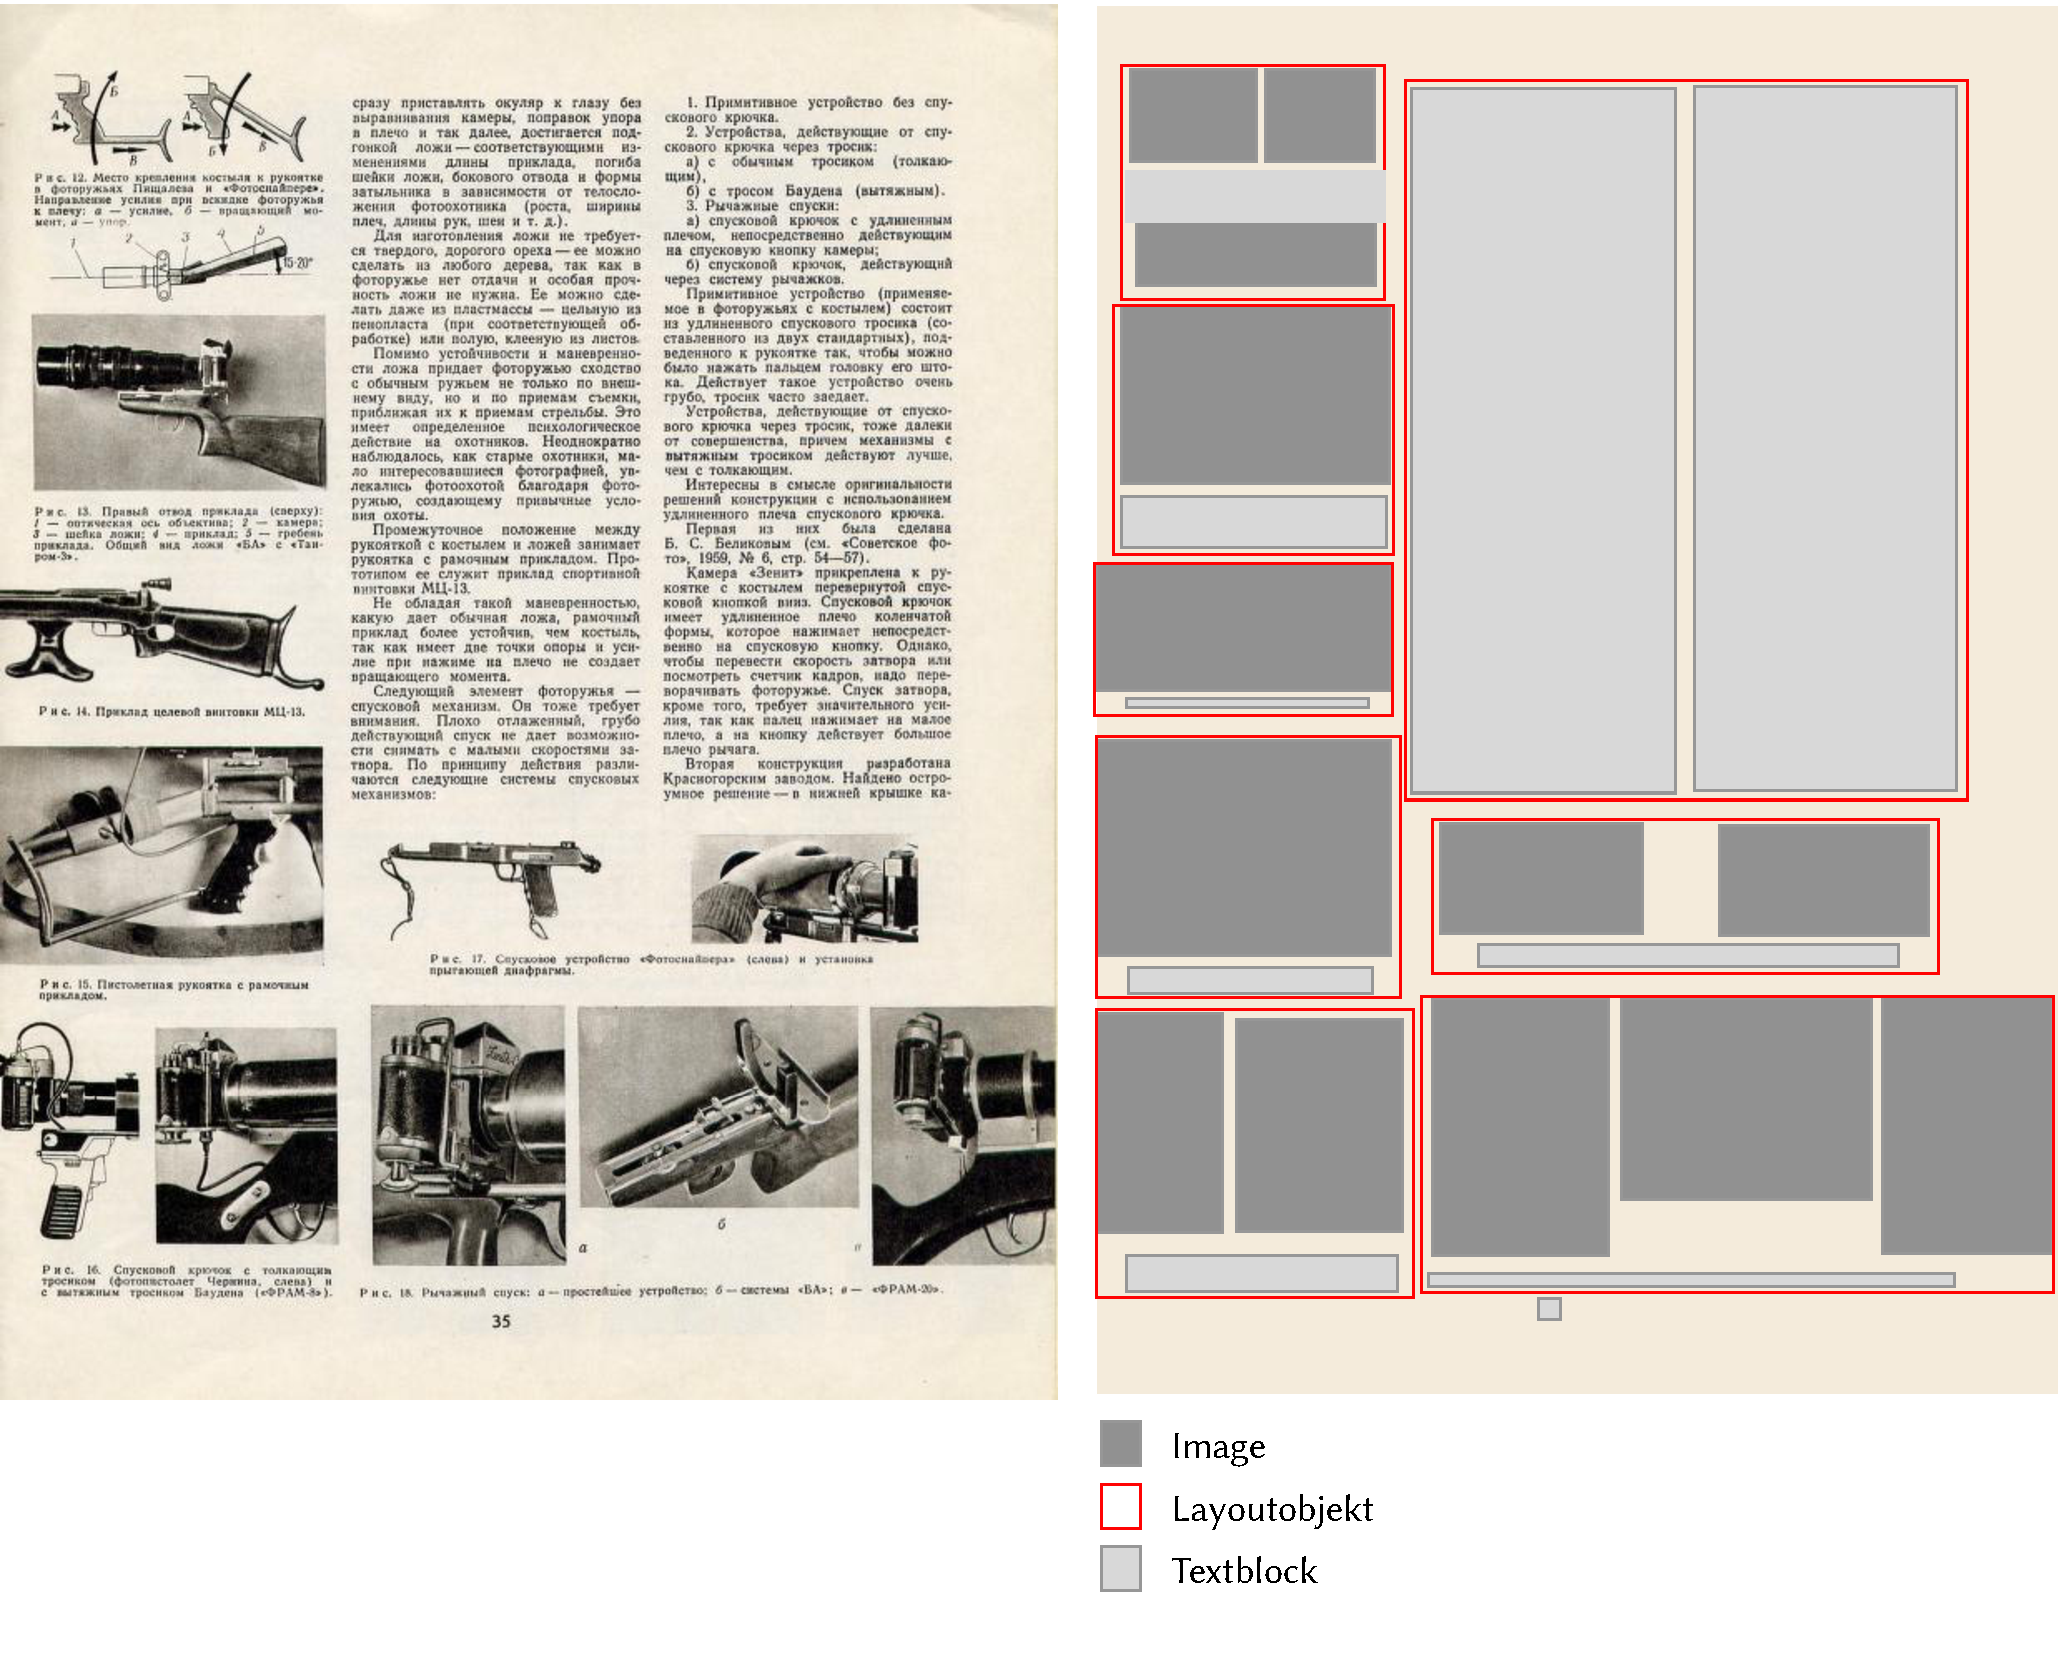
\includegraphics[width=\textwidth,keepaspectratio]{img/annotation_beispiel1.pdf}
\caption{ (links) Beispielseite aus einem Fotomagazin \cite{__1967}
          (rechts) Eine mögliche Annnotation}
\end{figure}
% \begin{marginfigure}
%     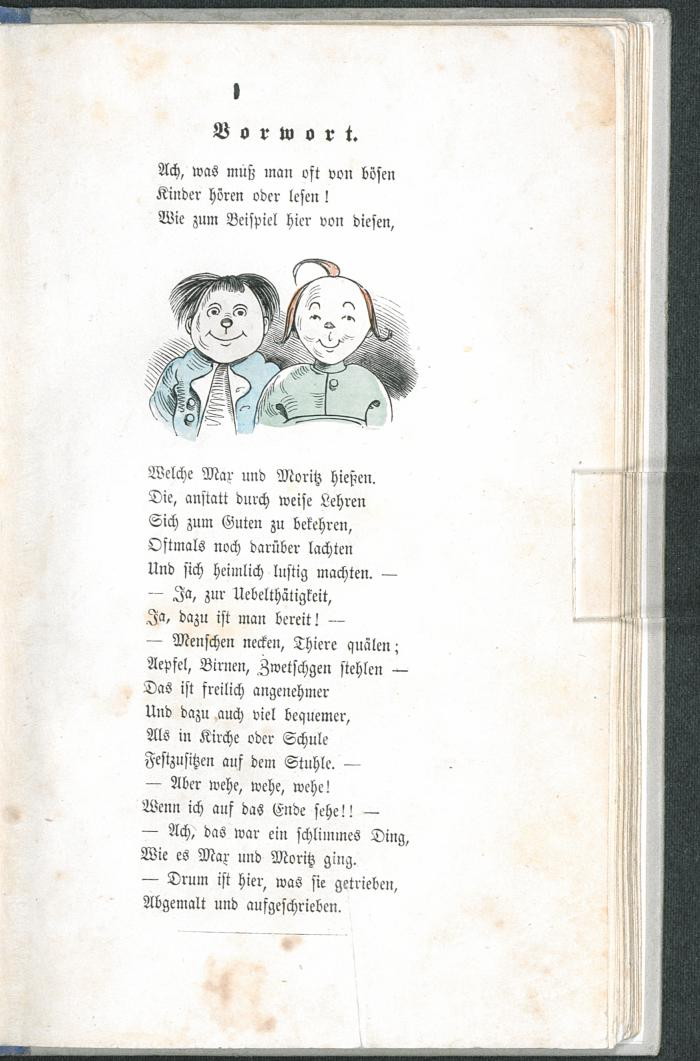
\includegraphics[width=\textwidth]{img/beispiel_text_bild.jpeg}
%     \caption{Ein Scan einer Buchseite mit Illustration\cite{wilhelm_busch_max_1865}}
%     \label{fig:busch} 
% \end{marginfigure}


\section{Zielstellung}
Das Ziel der Arbeit ist die Entwicklung einer Methode zur Klassifizierung von Dokumentinhalten um automatisch Metadaten zu erzeugen. 

Machinelles Lernen (ML) ist eine offensichtliche Wahl für Klassifizierungsprobleme. Für die Aufgabe der Bildklassifikation liefern künstliche Neuronalle Netze derzeit die besten Ergebnisse\cite{rodrigo_benenson_classification_2016}
Die Klasse der ``regional Convolutional Neural Networks'' (sieh z.B. \cite{girshick_region-based_2016}) ist in der Lage auf Basis eines CNN Bildregionen zu klassifizieren und zu segmentieren. 

Die besten Ergebnisse werden mit ``supervised learning'' Verfahren erreicht. 
Solche Verfahren profitieren ernorm von großen annotierten Datensätzen, welche 
für die hier genannte Problemstellung nur begrenzt vorliegen.
Um dieses Problem zu Lösen müssen in dieser Arbeit mehrere Ansätze kombiniert werden.
CNN können  sehr generische Bildrepräsentationen liefern \cite{razavian_cnn_2014}. 
Deswegen können bereits trainierte NN ``zweckentfremdet'' werden. Deshalb soll untersucht werden welche anderen Datensets für das Training verwendet werden können. 
Zum anderen ist es möglich NN-Klassifizierer auf großen Mengen unannotierten Daten zu trainieren \cite{le_building_2013}.



Für einen effektiven Einsatz von ML müssen auch Werkzeuge programmiert werden um die vorhandenen Daten zu visuallisieren 
und (semi)manuellel zu klassifizieren. 
Ohne diese Vorarbeit ist eine Evaluierung der Ergebnisse nur schwer möglich. 




\begin{enumerate}
	\item Beschreibung des Umfangs der Digitalen Sammlung
	\item Theorieteil über Neuronale Netze 
	\item Erstellung von Evaluierungsdaten
	\item Auswahl von geeigneten Architekturen für NN
	\item Parallelisierung der Datenverarbeitung
	\item Evaluierung und Visuallisierung der Ergebnisse
\end{enumerate}

% \nobibliography{/Developer/zotero/library.bib}
% \bibliographystyle{alpha}
\printbibliography{}
\end{document}
